\documentclass[ddc nogerman]{tudbeamer}
\usepackage[utf8]{inputenc}
\usepackage[english]{babel}

\usepackage[normalem]{ulem}
\usepackage{graphicx}

% the content
\begin{document}

\einrichtung{Department of Computer Science}
\institut{Institute for System Archticture}
\professur{Chair for Computer Networks}

\title{Application Development for Mobile and Ubiquitous Computing}
\subtitle{Seminar Task First Presentation}
\author{Alexandra Weiß, Gilbert Röhrbein}

\maketitle

\section{Bluemote}
\begin{frame}
    \makebox[\textwidth]{\centering \Huge \textbf{ Bluemote } }
\end{frame}

\begin{frame}
    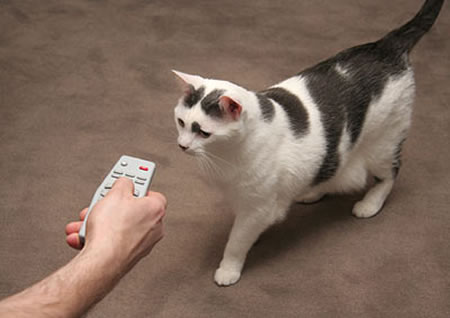
\includegraphics[height=\textheight]{img/remotecat.jpg}
\end{frame}

\section{Application Scenario}
\begin{frame}
    \begin{itemize}
        \item mobil remote control for stationary devices
        \item do the next presentation with it!
        \item watch a movie on a PC while sitting on a couch
        \item be easy (for developers) to adept to new devices
    \end{itemize}
\end{frame}

\section{Technologies}
\begin{frame}
    \begin{itemize}
        \item we have an Android 2.1 phone
        \item we have PCs
        \item Bluetooth instead of WLAN for communication
        \item\sout{act as a Bluetooth HID keyboard}
        \item emulate keys on the PC via little bluetooth server
        \item communicate via Bluetooth RFCOMM
    \end{itemize}
\end{frame}

\begin{frame}
    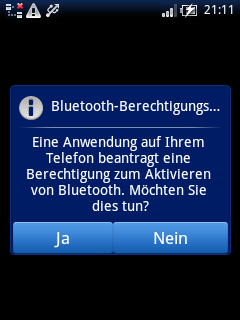
\includegraphics[height=\textheight]{img/btauth.jpg}
\end{frame}

\begin{frame}
    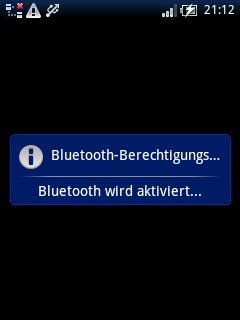
\includegraphics[height=\textheight]{img/btactivate.jpg}
\end{frame}

\begin{frame}
    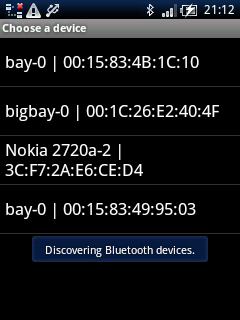
\includegraphics[height=\textheight]{img/choosedevice.jpg}
\end{frame}

\begin{frame}
    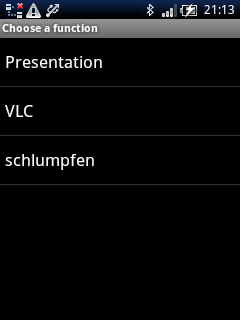
\includegraphics[height=\textheight]{img/choosefunction.jpg}
\end{frame}

\section{Challenges}
\begin{frame}
    \begin{itemize}
        \item seamless integration
        \begin{itemize}
            \item connect automatically to known devices
            \item start last used remote control function
            \item\sout{no change on the stationary device}
        \end{itemize}
        \item\sout{seamless integration}
        \begin{itemize}
            \item little bluetooth server necessary
            \item connect a USB stick with it to the PC
        \end{itemize}
        \item context awareness
        \begin{itemize}
            \item pause media player on call
        \end{itemize}
        \item extensible software
        \begin{itemize}
            \item easy (not hacky) addition of remote control functions
        \end{itemize}
    \end{itemize}
\end{frame}

\section{Work plan}
\begin{frame}
    \begin{itemize}
        \item prototype and learn more about Android SDK
        \\ \hfill
        \item presentation remote control function
        \item media player (VLC) remote control function
        \item movie night (gathering bug reports)
        \item fixing bugs, stabilize
        \\ \hfill
        \item if there is time, implementing first known HID keyboard service
            for Android phones
    \end{itemize}
\end{frame}

\begin{frame}
    
\includegraphics[height=\textheight]{img/endcat.jpg}
\end{frame}

\end{document}

